\documentclass[11pt,fleqn]{article} 
\usepackage[margin=0.8in, head=0.8in]{geometry} 
\usepackage{amsmath, amssymb, amsthm}
\usepackage{fancyhdr} 
\usepackage{palatino, url, multicol}
\usepackage{graphicx, pgfplots} 
\usepackage[all]{xy}
\usepackage{polynom,tabularx} 
\usepackage{enumerate}
\usepackage{framed}
\usepackage{setspace}
\usepackage{array}
\usepackage{pgf,tikz}
\usepackage{mathrsfs}
\usetikzlibrary{arrows}

\usetikzlibrary{calc}

\pgfplotsset{compat=1.6}

\pgfplotsset{soldot/.style={color=blue,only marks,mark=*}} \pgfplotsset{holdot/.style={color=blue,fill=white,only marks,mark=*}}

\renewcommand{\headrulewidth}{0pt}
\newcommand{\blank}[1]{\rule{#1}{0.75pt}}
\newcommand{\bc}{\begin{center}}
\newcommand{\ec}{\end{center}}
\newcommand{\be}{\begin{enumerate}}
\newcommand{\ee}{\end{enumerate}}

\renewcommand{\d}{\displaystyle}



\pagestyle{fancy} 
%\lfoot{Uses a calculator}
\rfoot{Review: Chapters 3 \& 4}

\begin{document}

\vspace*{-0.7in}

\begin{center}
  \large
  \sc{Review of Chapters 3 \& 4}\\
\end{center}


\bc Summary of Topics \ec
Chapter 3\\
\begin{itemize}
	\item Sections 1-6 primarily involve derivative rules. You will \emph{not} be explicitly tested on ``can you take a derivative'', but you will need to be able to accurately compute derivatives to answer all the problems. 
	\item Section 5 involves implicilty defined functions. You are expected to be able to use implicit differentiation to, for example, find the equation of a tangent line to an implicitly defined curve at a given point.
	\item Sections 7 and 8 focus on applications of the derivative in science and particularly to exponential growth and decay. Position, velocity and acceleration were again discussed. The overall emphasis is on \emph{interpretation} of the derivative in the context of an applied problem.
	\item Section 9 Related Rate Problems. In these problems you are always taking the derivative implicitly with respect to time and almost always seeking of find a rate of change at a particular instant.
	\item Section 10 Linear Approximations and Differentials. The crucial idea here is that the derivative can be used to estimate function-values or changes in function-values.
	\item Section 11 we did not cover.
\end{itemize}

Chapter 4\\
\begin{itemize}
	\item Section 1 makes a careful study of the ideas of local/absolute maximum/minimum and the difference between an extreme value ($y$-value) and where it occurs ($x$-value).
	\item Section 4.2 The Mean Value Theorem. Know, roughly, what it says and be able to draw a picture.
	\item Section 4.3 discussed how the sign of $f'$ and $f''$ can tell us things about $f$ such as intervals on which $f$ is increasing, decreasing, concave up, concave down, local/absolute extreme values.
	\item Section 4.4 involved L'H\^{o}pital's Rule. Recall that before using this rule one should make sure it applies.
	\item Section 4.5 put a whole bunch of Calculus together to sketch a graph. In addition to topics from Section 1 and 2, we also included things like $x$- and $y$-intercepts, vertical and horizontal asymptotes, and the function's domain.
	\item Section 4.6 was not discussed.
	\item Section 4.7 involved Optimization. Recall that by this time we have a clear  understanding of how the  domain of the function may determine the techniques we use to determine the answer. 
	\item Section 4.8 will be discussed at the end of the semester and will not appear on this midterm.
	\item Section 4.9 involves antiderivatives.
\end{itemize}

Note that the problems provided below are not necessarily comprehensive; they are intended to remind you of the sorts of problems we have discussed, but there may be other problems on the Midterm that don't look just like these!
%page 1
\newpage
\begin{enumerate}
%page 1
%linearization
\item Find the linearization of $f(x)=\sqrt{x}$ at $a=4$ and use it to estimate $\sqrt{4.1}$ and $\sqrt{3.8}$.
\vfill
\item Find the differential of $y=\sqrt{x}$ and use it to estimate how much $y$ will change as $x$ changes from $x=4$ to $x=4.1.$
\vfill
%lhop

\item If the \fbox{{\bf derivative}} of a function is shown below, identify all local maxima, minima, intervals of increase and decrease, intervals of concave up and concave down, and inflection points.

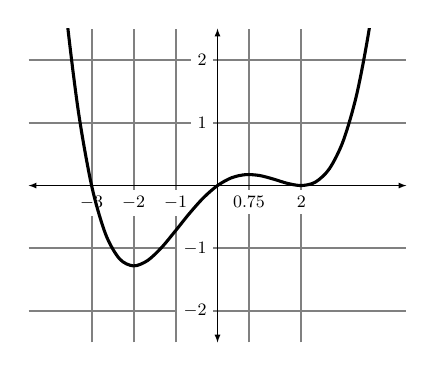
\begin{tikzpicture}[scale=0.7]
\begin{axis}[grid style={line width=.1pt, draw=black!50},grid=both,major grid style={line width=1pt,draw=black!50},
    xmin=-4.5,xmax=4.5,
    ymin=-2.5,ymax=2.5,
    xtick={-3, -2,-1, 0, .75, 2},ytick={},
    minor tick num=0,
    enlargelimits={abs=0},
    ticklabel style={font=\small,fill=white},
    axis lines=middle,
    axis line style={latex-latex},
    xlabel style={at={(ticklabel* cs:1)},anchor=north west},
    ylabel style={at={(ticklabel* cs:1)},anchor=south west}
]

\addplot[<->,domain=-4:4,ultra thick, smooth=100] {1/25*(x-2)^(2)*(x+3)*(x)};
\end{axis}
\end{tikzpicture}

\item Evaluate the following limits. Show your work. 
\be
\begin{multicols}{2}
\item $\d \lim_{x \to 0} \frac{1+x- e^x}{\sin x}$
\item  $\d \lim_{x \to\infty} x \ln (1+\frac{2}{x})$
\end{multicols}
\vspace{2.5in}
\ee
\newpage

%max and min on closed interval
\item 
\be
\item What are critical numbers of a function $f$?
\vspace{1in}
\item How do you find the absolute maximum and minimum of a function $f$ on a
  closed interval? (Assume $f$ is continuous on the interval.)
  \vspace{1in}
  \item Find the critical numbers of $f(x) = \sin(x) +
\sec(x)$ in $[-2\pi, \pi]$.
\ee
\vfill
%Mean Value Theorem
\item 
\be
\item State the Mean Value Theorem and draw a picture to illustrate it.
\vspace{2in}
\item Determine whether the Mean Value Theorem applies
to $f(x) = x(x^2 - x - 2)$ on $[-1, 1]$. If it can be applied find all
numbers that satisfy the conclusion of the Mean Value Theorem. 
\ee
\vfill
\newpage

\item Consider $f(x) = 2x- 2 \cos x$ on the interval $[- \pi, 2\pi]$
\be
 \item Find the open intervals on which the function is increasing or
    decreasing. \vfill
  \item Apply the first derivative test to identify all relative
    extrema. Classify each as a local maximum or local minimum.
    \vskip0.5in
  \item Find the open intervals on which the function is concave up or
    concave down.\vfill
      \item Find the inflection points.  \vskip0.5in
%  \item Describe the long-term behavior of the function.
%\vskip0.5in
\item What are the absolute maximum and minimum values of the function on the interval?
\vfill
  \item Sketch the graph.
  \ee
%  \vfill

\begin{center}
\begin{tikzpicture}
\draw[<->] (-6,0) -- (6,0);
\draw[<->] (0,-3) -- (0,3);
\end{tikzpicture}
\end{center}
  
  \newpage
  \item Find the rectangle of maximum area that can be inscribed inside the region bounded above by $y=20-x^2$ and bounded below by the $x$-axis. (Assume the base of the rectangle lies on the $x$-axis.) Begin by sketching a picture and labelling useful information.
  
  \vfill
  
  \vfill
  
  \vfill
  
\item Find the equation of the tangent line to the function $x^{3}+y^{3} = 6xy$ at the point $(3,3)$.

\vfill

\vfill

\item %review problems #101
 The angle of elevation of the sun is decreasing at a rate of 0.25 radians/hour. How fast is the shadow cast by a 400 foot tall building increasing when the angle of elevation of the sun is $\frac{\pi}{6}$ radians?
 \vfill 
  
  

%\item Find the domain of the function $f(x)=\frac{\sin(5x)}{x^2+x}$ and identify any vertical or horizontal asymptotes. Justify your answers.\\
%
%\vspace{2.5in}

%max and min on closed interval
%\item $f(x)=(x-4)\sqrt[3]{x}=x^{4/3}-4x^{1/3}; \quad f'(x)=\frac{4(x-1)}{3x^{2/3}}; \quad f''(x) = \frac{4(x+2)}{9x^{5/3}}.$
%\be
%  \item Find the critical numbers of $f(x).$
%  \vfill
%   \item Find the open intervals on which the function is increasing or
%    decreasing. \vfill
%    
%    \item Classify all critical points -- using the \textbf{first derivative test}.  \vfill
%    \newpage
%    From the other side: $f(x)=(x-4)\sqrt[3]{x}=x^{4/3}-4x^{1/3}; \quad f'(x)=\frac{4(x-1)}{3x^{2/3}}; \quad f''(x) = \frac{4(x+2)}{9x^{5/3}}.$
%    \item Classify all critical points -- using the \textbf{second derivative test}.  \vfill
%    
%    
%
%  \item Find the open intervals on which the function is concave up or
%    concave down.  \vfill
%    
%  \item Find the inflection points.   \vfill
%  
%  \item Sketch the graph.
%  \vfill
%\ee
%\ee
%
%\newpage

%page 2
%related rate
%\item A paper cup has the shape of a cone with height 10 cm and radius 3 cm (at the top). If water is poured into the cup at a rate of $2\: \text{cm}^3/\text{sec}$, how fast is the water level rising when the water is 5 cm deep? (Volume of a cone is: $V=(1/3) \pi r^2 h.$)
%\vfill
%\newpage
%page 5
%\item Find the dimensions of the rectangle of maximum area that can be inscribed in an equilateral triangle of side 20 cm if one side of the rectangle likes on the base of the triangle.
%\vfill
%Mean Value Theorem
%\item 
%\be
%\item State the Mean Value Theorem and draw a picture to illustrate it.
%\vspace{2in}
%\item Determine whether the Mean Value Theorem applies
%to $f(x) = x(x^2 - x - 2)$ on $[-1, 1]$. If it can be applied find all
%numbers that satisfy the conclusion of the Mean Value Theorem. 
%\ee
%\vfill
%\item Complete two iterations of Newton's Method to estimate a solution to $x^7+4=0$. Use $x_1=-1.$
\vfill
\end{enumerate}
\end{document}






